% Rebuild: xelatex -no-pdf -interaction=nonstopmode persistent-seg.tex
%          dvisvgm --no-fonts --exact-bbox persistent-seg.xdv -o persistent-seg.svg
\def\pgfsysdriver{pgfsys-dvisvgm.def}
\documentclass[tikz,border=4pt]{standalone}
\usetikzlibrary{arrows.meta,backgrounds}
\begin{document}
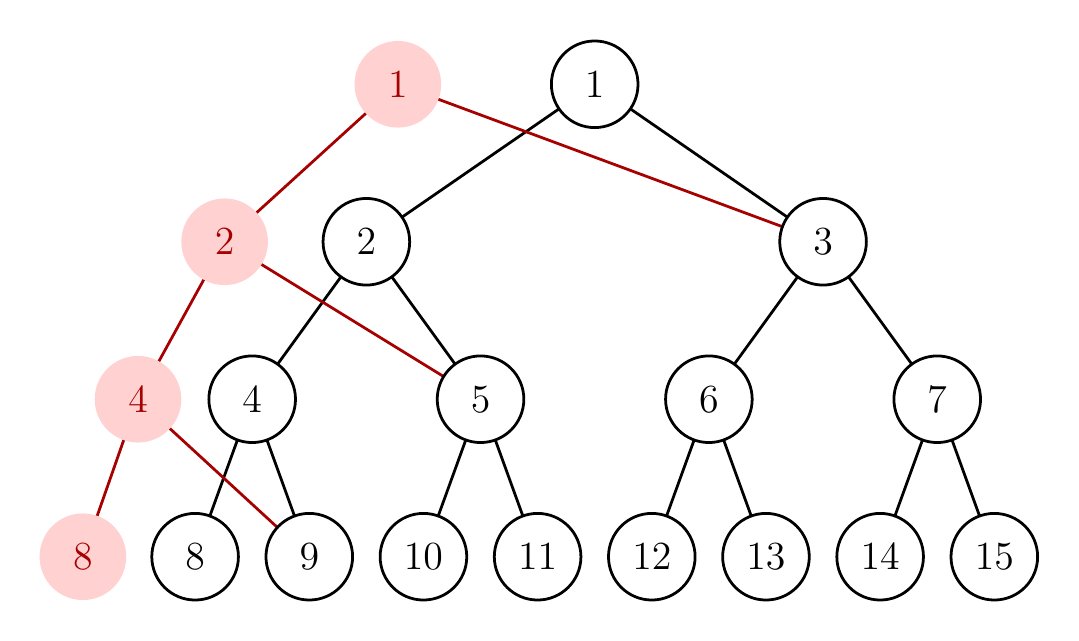
\begin{tikzpicture}[background rectangle/.style={fill=white},show background rectangle,x=1cm,y=1cm,line width=1pt,
  vertex/.style={circle,draw,fill=white,minimum size=11mm,inner sep=0pt,font=\Large},
  copied/.style={vertex,draw=none,fill=red!18,text=red!65!black}]
% Original heap-style numbers identify corresponding nodes, not stored counts.
\coordinate (n1) at (6.5,6);
\coordinate (n2) at (3.6,4);
\coordinate (n3) at (9.4,4);
\coordinate (n4) at (2.15,2);
\coordinate (n5) at (5.05,2);
\coordinate (n6) at (7.95,2);
\coordinate (n7) at (10.85,2);
\coordinate (n8) at (1.425,0);
\coordinate (n9) at (2.875,0);
\coordinate (n10) at (4.325,0);
\coordinate (n11) at (5.7749999999999995,0);
\coordinate (n12) at (7.225,0);
\coordinate (n13) at (8.675,0);
\coordinate (n14) at (10.125,0);
\coordinate (n15) at (11.575000000000001,0);
\draw (n1) -- (n2) (n1) -- (n3);
\draw (n2) -- (n4) (n2) -- (n5);
\draw (n3) -- (n6) (n3) -- (n7);
\draw (n4) -- (n8) (n4) -- (n9);
\draw (n5) -- (n10) (n5) -- (n11);
\draw (n6) -- (n12) (n6) -- (n13);
\draw (n7) -- (n14) (n7) -- (n15);
\coordinate (c1) at (4,6);
\coordinate (c2) at (1.8,4);
\coordinate (c4) at (0.7,2);
\coordinate (c8) at (0,0);
\draw[red!65!black] (c1) -- (c2);
\draw[red!65!black] (c1) -- (n3);
\draw[red!65!black] (c2) -- (c4);
\draw[red!65!black] (c2) -- (n5);
\draw[red!65!black] (c4) -- (c8);
\draw[red!65!black] (c4) -- (n9);
\node[vertex] at (n1) {1};
\node[vertex] at (n2) {2};
\node[vertex] at (n3) {3};
\node[vertex] at (n4) {4};
\node[vertex] at (n5) {5};
\node[vertex] at (n6) {6};
\node[vertex] at (n7) {7};
\node[vertex] at (n8) {8};
\node[vertex] at (n9) {9};
\node[vertex] at (n10) {10};
\node[vertex] at (n11) {11};
\node[vertex] at (n12) {12};
\node[vertex] at (n13) {13};
\node[vertex] at (n14) {14};
\node[vertex] at (n15) {15};
\node[copied] at (c1) {1};
\node[copied] at (c2) {2};
\node[copied] at (c4) {4};
\node[copied] at (c8) {8};
\end{tikzpicture}
\end{document}
